\chapter{Logik und Unterlagen}
Im Laufenden Semester werden wir viele mathematische Beweise einführen. Heute werden wir uns mit der Mathematische Logik beschäftigen. \\

In der Mathematik stossen wir auf gewisse Grundannahmen, ``Axiome'', die wir als gegeben ansehen. Eine dieser Annahmen ist der 
\subsection*{Satz vom ausgeschlossenen Dritten}
Eine zulässige mathematische Aussage ist entweder wahr oder falsch, jedoch nie beides zugleich.
\subsubsection*{Beispiel}
\begin{enumerate}
	\item $5<7$ Wahr
	\item $4<2$ Falsch
\end{enumerate}
In der wirklichen Welt ist es anders. Ist z.B. ``Mathematik ist schön'' wahr oder falsch?\\

Mit Aussagen kann man ``rechnen''. Wir führen nun ein paar geläufige Notationen der Logik ein:\\
\\
Seien $A,B$ Aussagen
\begin{itemize}
\item $A$ und $B$ wird mit $A\land B$ bezeichnet
\item $A$ oder $B$ wird mit $A\lor B$ bezeichnet
\end{itemize}
\subsubsection*{Folgerung (eine wahre Implikation)}
\begin{itemize}
\item Aus $A$ folgt $B$ wird mit $\to$ bezeichnet
\item Wenn $A$, dann auch $B$
\item Die Negation der Aussage $A$ wird mit $\lnot A$ bezeichnet
\item $A$ ist äquivalent zu $B$ wird mit $A\Leftrightarrow B$ bezeichnet
\item $\left(A\to B\right)\land \left( B\to A\right)$ $A$ wahr genau dann, wenn $B$ wahr ist.
\end{itemize}

\subsubsection*{Bemerkung}
Die Folgerung ist transitiv. Wenn wir wissen, dass $A\to B$ und $B\to C$, dann wissen wir dass $A\to C$.


\subsection*{Prinzip des Mathematischen Beweises}
Wir können aus eine Kette von Folgerungen \[A\to B \to C \dots \to S\]
einen mathematischen ``Satz'' $S$ aus einen Annahme $A$ herleiten. (Ein Beweis ist eine Folge von Implikationen von Aussagen). 
\subsubsection*{Kontraposition (Umkehrschluss)}

$A\to B$ ist gleichbedeutend mit $\lnot B\to\lnot A$.\\
Falls $A\to B$, so kann $A$ nicht wahr sein wenn $B$ falsch ist (weil wenn $A$ wahr ist, würde $B$ auch wahr sein).

\section{Prinzip des Indirekten Beweises}
Zum Beweis der Aussage $A\to B$ genügt es die Aussage $\lnot B\to\lnot A$ zu zeigen, oder die Annahme $A\land\lnot B$ zum Wiederspruch zu führen.

\subsection*{Indirekter Beweis}
Man fügt $\lnot B$ als Annahme hinzu und kommt nach einer Kette von erlaubten Schlüssen zu einer falschen Aussage.\\

\noindent Daraus schliesst man, dass die Zusatzannahme $\lnot B$ nicht wahr ist. 

\subsubsection*{Beispiel 1.1}
\begin{itemize}
\item $A=\text{''jede natürliche Zahl } n \text{ hat einen Nachfolger } n+1\text{''}$
\item $B=\text{''es gibt keine grösste natürliche Zahl''}$
\end{itemize}

\noindent Wir beweisen dass $B$ aus $A$ folgt . Nehmen wir an, dass $A$ wahr und $B$ falsch ist. \\

\noindent $\lnot B=$ es gibt eine grösste natürliche zahl $N_0''$, d.h $N_0>l$ für jedes $l \in \mathbb{N}$.\\

Mittels der Aussage $A$ wissen wir, dass $N_0$ einen Nachfolger $N_0 +1$ hat. Für diesen gilt $N_0+1>N_0$. Dies ist aber ein Wiederspruch.

\begin{definition}{1.1}
Eine Menge ist eine Zusammenfassung verschiedener Objekte zu einem Ganzen.\\
Die Objekte werden Elemente der Menge genannt. 
\end{definition}

Sei $A$ eine Menge, dann wird ``$a$ ist element von $A$'' mit ``$a\in A$'' bezeichnet.\\
Seien $A,B$ Mengen, dann wird ``jedes Element von $A$ ist ein Element von $B$'' mit ``$A\subset B$`` bezeichnet, und man sagt ``$A$ ist in $B$ enthalten'' (oder $A$ ist eine Teilmenge von $B$). \\

Falls zugleich $A\subset B$ und $B\subset A$ gilt, so sind $A$ und $B$ gleich und man schreibt $A=B$. 

\subsubsection*{Beispiele 1.2}
\begin{enumerate}
	\item Die Menge $\mathbb{N}=\{0,1,2,\dots\}$ der natürlichen Zahlen.
	\item Die leere Menge mit ``$\varnothing$'' bezeichnet. Sie ist in jeder Menge enthalten.
	\item Die Menge $\mathbb{Z}=\{\dots,-2,-1,0,1,2,\dots\}$ aller ganze Zahlen.
	\item Meistens werden Mengen nicht durch die Liste ihre Elemente gegeben, sondern durch bestimmte Eigenschaften ihrer Elemente definiert \[\mathbb{P}=\{2,3,4,5,7,11,13,\dots\}\] die Menge aller Primzahlen $\mathbb{P}:\{p\in\mathbb{N}\mid\text{ $p$ primzahl}\}$
\end{enumerate}
\section{Zwei Prinzipen}
Wir werden die folgenden zwei Beweismethoden häufig benutzen.

 \subsection*{1. Prinzip des Indirekten Beweises}
Zum Beweis der Aussage $A\to B$ genügt es, die Aussage $\lnot B\to\lnot A$ zu zeigen oder die Annahme $A\land\lnot B$ zum Wiederspruch zu führen.
\subsection*{2. Prinzip der Vollständigen Induktion}
Sei für jedes $n\in\mathbb{N}$ eine Behauptung $A(n)$ gegeben. Soll die Behauptung für alle natürlichen Zahlen $n\in\mathbb{N}$ bewiesen werden, so genügen dazu zwei Beweisschritte:
\begin{enumerate}[i)]
\item Der Beweis von $A(0)$
\item Für jedes $n\in\mathbb{N}$, der Beweis von $A(n+1)$ unter der Voraussetzung, dass $A(n)$ gilt. 
\end{enumerate}
Oft gelten aber Behauptungen nicht von $n=0$. \\
Soll die Gültigkeit von $A(n)$ für alle $n\geq m$ bewiesen werden so genügen wieder zwei Schritte:
\begin{enumerate}[i)]
	\item Beweis von $A(m)$
	\item Für jedes $n\geq m$ impliziert $A(n)$ die Behauptung $A(n+1)$
\end{enumerate}
Das Prinzip der vollständigen Induktion ist genau wie ein Dominoeffekt.\\

Sie stellen alle Dominosteine  auf, einen nach dem anderen. Falls der erste Dominostein fällt ($A(1)$ wahr) und falls wir die Dominosteine genug nah nebeneinander gestellt haben, so dass ein fallender Dominostein den nächsten trifft ($A(k)\to A(k+1)$), dann wissen wir, dass alle Dominosteine fallen. 

\subsubsection*{Beispiel 1.3 (Induktion)}
\begin{enumerate}
\item Für alle $n\geq 1$ gilt: \[A(n): \quad 1+3+5+\dots (2n-1)=n^2\] Beweis mittels vollständiger Induktion
\begin{enumerate}[i)]
\item $A(i)$ lautet $1=1^2$ und gilt.
\item Sei $n\geq 1$. Annahme: $A(n)$ gilt. Die linke Seite der Identität $A(n+1)$ ist \[1+3+\dots +(2n-1)+(2n+1)=n^{2}+(2n+1)=(n+1)^2\] womit $A(n+1)$ bewiesen ist.
\end{enumerate}
\item Als zweites Beispiel der vollständigen Induktion beweisen wir den Fundamentalsatz von Euklid:
\subsubsection*{Satz 1.4}
Jede natürliche Zahl $n\geq 2$ ist ein Produkt von Primzahlen, welches bis auf die Reihenfolge der Faktoren eindeutig ist. Wir werden uns hier aber nicht mit der Eindeutigkeit befassen.
\subsubsection*{Beweis}
Sei $A(n)$ die Aussage: Jede natürliche Zahl $m$ mit $2\leq m\leq n$ ist ein Produkt von Primzahlen
\begin{enumerate}[i)]
\item $A(2)$ gilt, denn $2$ ist eine Primzahl.
\item Sei $n\geq 2$. Wir nehmen an, dass $A(n)$ gilt. Für $n+1$ gibt es zwei Möglichkeiten
\begin{enumerate}[a)]
\item $n+1$ ist eine Primzahl und somit gilt $A(n+1)$ 
\item $n+1$ ist keine Primzahl d.h. es gibt ein $2\leq a\leq n$ welches $n+1$ teilt. Dann ist $b\defeq\frac{n+1}{a}$ auch ganzzahlig und zudem ist $2\leq b\leq n$ erfüllt. Aus $A(n)$ folgt, dass sowohl $a$ wie $b$ ein Produkt von Primzahlen sind. Somit ist auch $n+1=ab$ ein Produkt von Primzahlen. 
\end{enumerate}
\end{enumerate}
\end{enumerate}
\subsubsection*{Satz 1.5}
Die Menge $\mathbb{P}$ der Primzahlen ist unendlich.
\subsubsection*{Beweis}
Nehmen wir das Gegenteil ``$\mathbb{P}$ ist endlich'' an, d.h. $\mathbb{P}=\{p_1,p_2,\dots,p_m\}$ in aufsteigender Folge; also $p_1=2,p_2=3,p_3=5,p_4=7,\dots$. Wir betrachten die Zahl $k=p_1 p_2\dots p_i \dots p_m+1$. Aus Satz 1.4 folgt, dass eine Primzahl $p_i$ (aus der Liste $\{p_1 ,\dots , p_{m}\}$) existiert, mit $p_i$ teilt $k$. Da $p_i$ offensichtlich $p_1 p_2\dots p_i \dots p_m$ teilt, folgt dass $p_i$ die Restzahl $k-p_1\dots p_{m}=1$ teilt. Das ist ein Widerspruch. 

\subsection*{Teilbarkeit}
\subsubsection{Formale Definition}
Eine ganze Zahl $a$ teilt eine ganze Zahl $b$ genau dann, wenn es eine ganze Zahl $n$ gibt, für die $an=b$ ist. \\
\begin{center}
\begin{tabular}{l|l}
Man sagt dann (Synonyme) & Man schreibt \\\hline 
$a$ teilt $b$ & $a\mid b$\\
$a$ ist Teiler von $b$ & ~\\
$b$ ist teilbar durch $a$ & ~\\
$b$ ist Vielfaches von $a$ & ~\\
\end{tabular}
\end{center}

\subsubsection*{Eigenschaften der Teilbarkeit}
\begin{itemize}
\item Gilt $a\mid b$ und $b\mid c$, so folgt $a\mid c$
\item Für $k\in\mathbb{Z}\backslash\{0\}$ gilt: $a\mid b\Longleftrightarrow ka\mid kc$ 
\item $a\mid b$ und $c\mid d\to ac\mid bd$
\item $a\mid b$ und $a\mid c\to a\mid kb+lc,\text{    für alle }l,k\in\mathbb{Z}$
\end{itemize}

\subsubsection{Formaler Beweis von Satz 1.5}

\begin{enumerate}
\item $k=\left( p_1 p_2\dots p_i \dots p_m \right)+1$\\
Es gibt eine Primzahl $p_i$ die $k$ teilt. $p_i\mid k$ mittels Satz 1.4.
\item Sei $b=p_1 p_2\dots p_i \dots p_m=$ Produkt aller Primzahlen. Sei $a=p_i$, $n=p_1 p_2 p_{i-1} p_{i+1} \dots p_m$. Dann $b=an$. Das bedeuted, dass $a$ ein Teiler von $b$ ist, d.h. $p_i\mid\left(p_1\dots p_m\right)$
\item $p_i\mid k$ und $p_i\mid \left(p_1\dots p_m\right) \to p_i \mid k-\left(p_1\dots p_m\right)=1$.\\
So erhalten wir einen Widerspruch.
\end{enumerate}

\subsubsection*{Bemerkung}
Letztes mal haben wir gesagt, dass ``jedes Element von $A$ ist auch Element von $B$'' ($\forall x,x\in A\to x\in B$) mit $A\subset B$ bezeichnet wird. Wir sagen auch ``$A$ ist in $B$ enthalten'' oder ``$A$ ist Teilmenge von $B$''. Falls $A\subset B$ und eine Element $b\in B$ existiert mit $b\not\in A$, so sagen wir ``$A$ ist eine ``eigentliche Teilmenge'' von $B$''. Manchmal schreiben wir $A\mathop  \subset \limits_{\not  = } B$ in diesem Fall. \\

Es gibt viele Bücher mit der folgenden Notation: ``jedes Element von $A$ ist ein Element von $B$'' wird mit $A\subseteq B$ bezeichnet. Und wenn $A\subseteq B$ und $A\not =B$ dann wird $A\subset B$ statt $A\mathop  \subset \limits_{\not  = } B$ benutzt. $A=B$ falls $x\in A\Leftrightarrow x\in B$. 

\subsubsection*{Satz}
$A=B \Leftrightarrow A\subset B$ und $B\subset A$ 
\subsubsection*{Beweis}
Annahme: $A=B$. Falls $x\in A$, dann gilt, mittels $A=B$, $x\in B$ und damit gilt auch $A\subset B$. Falls $x\in B$, dann gilt $x\in A$ (mittels $A=B$), und damit gilt $B\subset A$.\\

Wir haben bewiesen, dass $A=B \to A\subset B \text{ und } B\subset A$. \\
Nun nehmen wir $A\subset B$ und $B\subset A$ an. Damit möchten wir $A=B$ zeigen. \\

Sei $x\in A$. Mittels $A\subset B$ erhalten wir $x\in B$ und somit $x\in A \to x\in B$. (\textasteriskcentered)\\

Sei $x\in B$. Mittels $B\subset A$ erhalten wir $x\in A$ und somit $x\in B \to x\in A$. (\textasteriskcentered\textasteriskcentered)\\

(\textasteriskcentered) und (\textasteriskcentered\textasteriskcentered) $\to A=B$ per Definition. 

\section{Mengenoperationen}
Zunächst erinnern wir kurz an die Definitionen der elementaren Operationen auf Mengen. \\

\noindent Seien $A$ und $B$ Mengen. Wir können dann daraus folgende Mengen bilden:

\begin{itemize}
\item Die Vereinigung: $A\cup B=\{x\mid x\in A \lor x\in B\}$
\item Der Durchschnitt: $A\cap B=\{x\mid x\in A \land x\in B\}$
\item Die Differenz: $A\backslash B=\{x\mid x\in A \land x\not\in B\}$
\item Symmetrische Differenz: $A\bigtriangleup B=\left(A\backslash B\right) \cap \left(B\backslash A\right)=\left(A\cup B\right)\backslash\left(A\cap B\right)$
\end{itemize}

Wir haben dann folgende Eignschaften
\subsubsection*{Satz 1.6}
Seien $A,B,C$ Mengen. 
\begin{enumerate}
\item $A\cap B=B\cap A$; $A\cup B=B\cup A$\\
$A\cap \emptyset=\emptyset$; $A\cup \emptyset=A$\vspace{-4mm}
\subsubsection*{Bemerkung}
\begin{itemize}
    \item $\cup$ verhält sich wie $+$
    \item $\cap$ verhält sich wie die Multiplikation
    \item $\emptyset$ verhält sich wie das Nullelement
\end{itemize}
    \item $\left( A\cup B\right)\cup C=A\cup\left( B\cup C\right)$\\
    $\left( A\cap B\right)\cap C=A\cap\left( B\cap C\right)$
    \item $\left( A\cup B\right) \cap C=\left( A\cap C\right) \cup \left( B\cap C\right)$
\end{enumerate}



\subsubsection*{Beweis}
Einerseits gilt
\[
(A \cup B) \cap C = \{x \in X: x \in A \cup B \} \land \{ x \in X: x \in C\}
\]
Andererseits $(A \cap C) \cup ( B \cap C) = \{ x \in X: x \in A \cap C \} \lor \{ x \in X : x \in B \cap C \}$. Daraus folgt
\begin{align*}
(A \cup B ) \cap C &\subseteq (A \cap C) \cup (B \cap C) \\
(A \cap C ) \cup (B \cap C) &\subseteq (A \cup B) \cap C
\end{align*}
und somit sind die zwei Mengen gleich.

\begin{definition}{1.7}
Das Kartesische Produkt $A\times B$ der Mengen $A,B$ ist die Menge der geordneten Paare $(a,b)$ wobei $a\in A, b\in B$
\end{definition}

\subsubsection*{Beispiel}
$\mathbb{Z}\times\mathbb{Z}=\{(a,b):a\in\mathbb{Z},b\in\mathbb{Z}\}$. Falls $\mathbb{Z}$ als ``eindimensionales'' Gebilde dargestellt wird 

\begin{center}
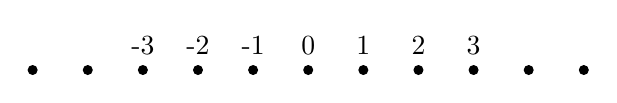
\begin{tikzpicture}[scale=0.7]


\draw	(0,0) node[anchor=south] {-3}
		(1,0) node[anchor=south] {-2}
		(2,0) node[anchor=south] {-1}
		(3,0) node[anchor=south] {0}
		(4,0) node[anchor=south] {1}
		(5,0) node[anchor=south] {2}
		(6,0) node[anchor=south] {3}
		
		;
\filldraw (2,-0.1) circle (0.08)
(1,-0.1) circle (0.08)
(0,-0.1) circle (0.08)
(-1,-0.1) circle (0.08)
(-2,-0.1) circle (0.08)
(2,-0.1) circle (0.08)
(3,-0.1) circle (0.08)
(4,-0.1) circle (0.08)
(5,-0.1) circle (0.08)
(6,-0.1) circle (0.08)
(7,-0.1) circle (0.08)
(8,-0.1) circle (0.08)
;
		
		
\end{tikzpicture}
\end{center}

So wird $\mathbb{Z}\times\mathbb{Z}$ als ``zweidimensionales'' Gebilde dargestellt 

\begin{center}
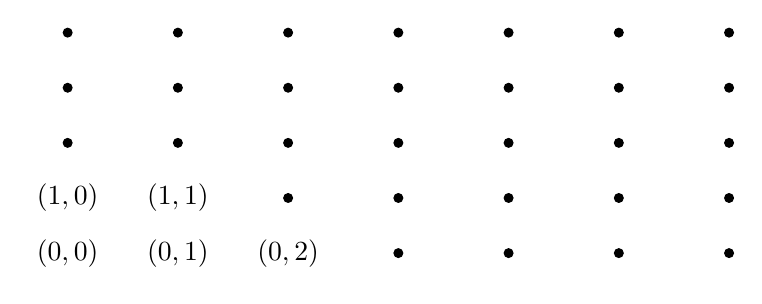
\begin{tikzpicture}[scale=0.7]


\draw	(0,0) node[] {$(0,0)$}
		(2,0) node[] {$(0,1)$}
		(4,0) node[] {$(0,2)$}
		(0,1) node[] {$(1,0)$}
		(2,1) node[] {$(1,1)$}
		;
\filldraw 
(0,2) circle (0.08)
(0,3) circle (0.08)
(0,4) circle (0.08)
(2,2) circle (0.08)
(2,3) circle (0.08)
(4,3) circle (0.08)
(6,3) circle (0.08)
(8,3) circle (0.08)
(10,3) circle (0.08)
(12,3) circle (0.08)
(4,2) circle (0.08)
(6,2) circle (0.08)
(8,2) circle (0.08)
(10,2) circle (0.08)
(12,2) circle (0.08)

(4,1) circle (0.08)
(6,1) circle (0.08)
(8,1) circle (0.08)
(10,1) circle (0.08)
(12,1) circle (0.08)
(10,0) circle (0.08)
(12,0) circle (0.08)

(2,4) circle (0.08)
(4,4) circle (0.08)
(6,4) circle (0.08)
(8,4) circle (0.08)
(10,4) circle (0.08)
(12,4) circle (0.08)
(6,0) circle (0.08)
(8,0) circle (0.08)
;
\end{tikzpicture}
\end{center}



Um die Operationen auf mehrere Mengen zu verallgemeinern, sind die folgenden Quantoren nützlich ($\ast$)
\begin{enumerate}
\item $\forall$ ``Für alle'' (Allquantor)
\item $\exists$ ``Es gibt'' (Existenzquantor)
\item $\exists !$ ``Es gibt genau ein''
\end{enumerate}
Sei nun $I$ eine beliebige Menge ($I$=Indexmenge) und sei für alle $i\in I$ eine Menge $A_i$ gegeben. Dann:
\begin{itemize}
\item $\mathop{\bigcup}\limits_{i \in I}{A_i} = \{x\mid \exists i\in I,x\in A_i\}$. Vereinigung besteht aus den Elementen $x$, für welche es ein $i\in I$ gibt, so dass $x$ zu $A_i$ gehört.
\item  $\mathop{\bigcap}\limits_{i \in I}{A_i} = \{x\mid \forall i\in I,x\in A_i\}$. Durchschnitt. 
\end{itemize}
Wir definieren das Kartesische Produkt endlich vieler Mengen $A_1 \dots A_n$: \[{A_1} \times {A_n} = \prod\limits_{i = 1}^n {{A_i} = \{ ({x_1}, \ldots, {x_n})\mid {x_i} \in {A_i}} \} \]

\subsubsection*{Satz 1.8}
Seien $A_1 \dots A_k \subset X, \; k\in \mathbb{N}$. Es gilt
\begin{enumerate}
\item \[{\left( {\bigcap\limits_{i = 1}^k {{A_i}} } \right)^c} = \bigcup\limits_{i = 1}^k {{A_i}^c} \]
\item \[{\left( {\bigcup\limits_{i = 1}^k {{A_i}} } \right)^c} = \bigcap\limits_{i = 1}^k {{A_i}^c} \]
\end{enumerate}
\subsubsection*{Beweis}
\begin{align*}
{\left( {\bigcap\limits_{i = 1}^k {{A_i}} } \right)^c}
  =&\left\{x \;| \; {x \in X \wedge x\not  \in \bigcap\limits_{i = 1}^k {{A_i}} } \right\} 
  = \left\{ x \;| \; {x \in X, \exists i \in \left\{ {1, \ldots ,k} \right\}:x\not  \in {A_i}} \right\}\\
 =&\bigcup\limits_{i = 1}^k {\left\{ x \;| \; {x \in X \wedge x\not  \in {A_i}} \right\}}   = \bigcup\limits_{i = 1}^k {A_i^c}
\end{align*}
und
\begin{align*}
{\left( {\bigcup\limits_{i = 1}^k {{A_i}} } \right)^c} 
=&\left\{x \;| \; {x \in X \wedge x\not  \in \bigcup\limits_{i = 1}^k {{A_i}} } \right\} 
= \left\{x \;| \; {x \in X, \forall i \in \left\{ {1, \ldots ,k} \right\}:x\not  \in {A_i}} \right\}\\
=&\bigcap\limits_{i = 1}^k {\left\{ {x \;| \;x \in X \wedge x\not  \in {A_i}} \right\}}  
= \bigcap\limits_{i = 1}^k {A_i^c} 
\end{align*}
\noindent (Siehe Analysis Serie 1, 1. Semester, Aufgabe 2.e)
\begin{enumerate}[($\ast$)]
\item Wir haben gesehen, dass wir manchmal eine Aussage verneinen müssen. Deshalb müssen wir lernen wie man Aussagen mit Quantoren verneinen kann.
\[\neg\left(\forall n:A(n)\right)\Leftrightarrow\left(\exists n:\neg A(n)\right)\]
\[\neg\left(\exists n:A(n)\right)\Leftrightarrow\left(\forall n:\neg A(n)\right)\]
\[\neg\left(\forall x\in \mathbb{R}:x^2\geq 0\right)\Leftrightarrow\exists x\in\mathbb{R}:x^2<0\]
\end{enumerate}
\section{Abbildungen}
Seien $X,Y$ Mengen. 

\begin{definition}{1.9}
Eine Funktion oder Abbildung $f:X\to Y$ der Menge $X$ in die Menge $Y$ ist eine Vorschrift (ein Gesetz) die (das) jedem Element $x\in A$ genau ein Element $y=f(x)\in Y$ zuordnet. \\

Es gibt verschiedene wichtige Objekte die in Zusammenhang mit einer Abbildung auftreten 
\begin{align*}
X &= \text{ \emph{Definitionsbereich} oder \emph{Definitionsmenge} (domain)} \\
Y&= \text{ \emph{Wertebereich} oder \emph{Zielmenge} (range)} \\
f(X) &=\{f(x)\mid x\in X\}\text{ ist das sog. \emph{Bild} oder die \emph{Bildmenge}} \\
f^{-1}(y) &= x\text{ heisst \emph{Urbild} von }y. \end{align*}
Der \emph{Graph} einer Funktion $f$ ist die Menge aller Paare $(x, f(x))$ wobei $x$ alle Elemente der Menge $X$ durchläuft. Er ist eine Teilmenge von $X \times Y$.
\[ Gr(f) \defeq \{ (x, f(x)) \mid x \in X\} \]
\end{definition}

\subsubsection*{Beispiel 1.10}
\begin{enumerate}
\item (Identität) Für jede Menge $\Romanbar{X}$, ist $id_X : \Romanbar{X} \to\Romanbar{X}$ definiert durch $id_{\Romanbar{X}}(x)=x, \forall x\in X$ 

\begin{center}
\begin{tikzpicture}[scale=0.5]
\draw (-2.5,0) ellipse (1.5 and 3);
\draw (2.5,0) ellipse (1.5 and 3);


\draw[-triangle 60]  (-2.5,2) parabola bend (-0.5,2) (2.8,1.3);


\draw[-triangle 60](-2.8,0) parabola bend (1,1) (3.2,0.5);
\draw[-triangle 60](-2,-1) parabola bend (0,-0.8) (2,-1);

\draw	(-1,3) node[anchor=east] {$X$}
		(4,3) node[anchor=east] {$X$};



\filldraw 
(-2.5,2) circle (0.08)
(-2.8,0) circle (0.08)
(-2,-1) circle (0.08)

(2.8,1.3) circle (0.08)
(3.2,0.5) circle (0.08)
(2,-1) circle (0.08)
;
\end{tikzpicture}
\end{center}



\item (Konstante) Sei $X$ Menge und $c\in \Romanbar{X}$. Die konstante Abbildung mit Wert $c$ ist $f(x)=c, \forall x \in \Romanbar{X}$  

\begin{center}
\begin{tikzpicture}[scale=0.5]
\draw (-2.5,0) ellipse (1.5 and 3);
\draw (2.5,0) ellipse (1.5 and 3);


\draw[-triangle 60]  (-2.5,2) parabola bend (-0.5,2) (3.2,0.5);


\draw[-triangle 60](-2.8,0) parabola bend (1,1) (3.2,0.5);
\draw[-triangle 60](-2,-1) parabola bend (3.2,0.5) (3.2,0.5);

\draw	(-1,3.1) node[anchor=east] {$\Romanbar{X}$}
		(4,3.1) node[anchor=east] {$\Romanbar{X}$}
		(3.9,0.1) node[anchor=east] {$C$}
		;

\filldraw 
(-2.5,2) circle (0.08)
(-2.8,0) circle (0.08)
(-2,-1) circle (0.08)


(3.2,0.5) circle (0.08)
;
\end{tikzpicture}
\end{center}


\item Seien $X,Y$ Mengen. Dann sind \\
\begin{tabular}{r  l c r l c }
$pr_x:$ & $X\times Y\to X $& ~ & $pr_y$: & $X\times Y\to Y$ \\
~& $(x,y)\mapsto x$ & ~& ~& $(x,y)\mapsto y$ \\
\end{tabular}\\
die Projektionen auf den ersten bzw. zweiten Faktor. 
\item Sinus \begin{align*} f:\mathbb{R}&\to\lbrack -1,1\rbrack \\ x &\mapsto \sin x \end{align*}
\item \begin{align*}f:\mathbb{R}&\to\mathbb{R} \\ x&\mapsto x^2+x\end{align*}
\end{enumerate}
\begin{definition}{1.11}
Sei $f:X\to Y$ eine Abbildung
\begin{enumerate}
\item $f$ heisst injektiv falls aus $f(x_1)=f(x_2)$ stets $x_1=x_2$ folgt, also falls jedes $y\in Y$ höchstens ein Urbild hat.
\item $f$ heisst surjektiv falls es für jedes $y\in Y$ ein $x\in X$ gibt mit $f(x)=y$ \[\forall y\in Y, \exists x\in X:f(x)=y\] Also wenn jedes Element $y\in Y$ mindestens ein Urbild hat. 
\item $f$ heisst bijektiv falls $f$ injektiv und surjektiv ist, d.h. falls jedes $y\in Y$ genau ein Urbild hat. 
\end{enumerate}
\end{definition}

\begin{multicols}{2}
[\subsubsection*{Beispiel 1.12}]
\begin{enumerate}
\item $id_{X}:X\to X$ bijektiv.
\item Eine konstante Abbildung \\
	$f:\Romanbar{X}\to X, x\mapsto c$ ist 
\begin{itemize}
\item injektiv $\Leftrightarrow \Romanbar{X}=\{ c\}$
\item surjektiv $\Leftrightarrow X=\{ c\}$
\end{itemize}
\item Die Projektionen 
\begin{itemize}
\item $pr_x : X\times Y\to X$ 
\item $pr_y : X\times Y\to Y$ 
\end{itemize}
sind stets surjektiv.
\item $f:\mathbb{R}\to\lbrack -1,1\rbrack$ \\
$x\mapsto \sin x$\\
Surjektiv, nicht injektiv
\columnbreak
\item $f:\mathbb{R}\to\mathbb{R}$\\
$x\mapsto x^2$\\
Nicht surjektiv\\
Nicht injektiv

\item $f:\mathbb{N}\to\mathbb{N}$\\
$n\mapsto 2n$\\
ist injektiv. $f(\mathbb{N})$ ist die Menge aller geraden Zahlen
\item Eine Menge $A$ hat $n$ Elemente falls es eine bijektive ${f:\{1,\dots,n\}\to A}$ gibt. Die Zahl $n$ wird dann die Kardinalität von $A$ genannt und mit $|A|$, gelegentlich auch mit $\#A$ bezeichnet.
\end{enumerate}
\end{multicols}

\begin{definition}{Kardinalität}
Wir sagen zwei Mengen $X$ und $Y$ sind gleichmächtig falls eine bijektive Abbildung $f:X\to Y$ existiert.
\end{definition}

Mit dem ersten Cantorschen Diagonalverfahren kann man die rationalen Zahlen abzählen, d.h.$ \mathbb{Q}$ und $\mathbb{N}$ sind gleichmächtig

\begin{center}
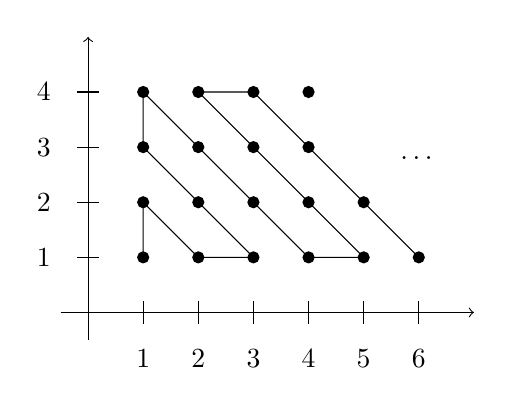
\begin{tikzpicture}[scale=0.7]

% horizontal axis
\draw[->] (-0.5,0) -- (7,0) node[anchor=north] {};
% labels
\draw	(-0.5,1) node[anchor=east] {1}
		(-0.5,2) node[anchor=east] {2}
		(-0.5,3) node[anchor=east] {3}
		(-0.5,4) node[anchor=east] {4}
		
		(1,-0.5) node[anchor=north] {1}
		(2,-0.5) node[anchor=north] {2}
		(3,-0.5) node[anchor=north] {3}
		(4,-0.5) node[anchor=north] {4}
		(5,-0.5) node[anchor=north] {5}
		(6,-0.5) node[anchor=north] {6}
		
		(6,3) node[anchor=north] {\dots}
		
		;
%lines for labes
\draw (-0.2,1) -- (0.2,1)
(-0.2,2) -- (0.2,2)
(-0.2,3) -- (0.2,3)
(-0.2,4) -- (0.2,4)

(1,-0.2) -- (1,0.2)
(2,-0.2) -- (2,0.2)
(3,-0.2) -- (3,0.2)
(4,-0.2) -- (4,0.2)
(5,-0.2) -- (5,0.2)
(6,-0.2) -- (6,0.2);

%draw dots
\filldraw[color=black] (1,1) circle (0.1)
(2,1) circle (0.1)
(3,1) circle (0.1)
(4,1) circle (0.1)
(5,1) circle (0.1)
(6,1) circle (0.1)
(1,2) circle (0.1)
(2,2) circle (0.1)
(3,2) circle (0.1)
(4,2) circle (0.1)
(5,2) circle (0.1)
(1,3) circle (0.1)
(2,3) circle (0.1)
(3,3) circle (0.1)
(4,3) circle (0.1)
(1,4) circle (0.1)
(2,4) circle (0.1)
(3,4) circle (0.1)
(4,4) circle (0.1)
;

% vertical axis
\draw[->] (0,-0.5) -- (0,5) node[anchor=east] {};

%connection through points
\draw (1,1)--(1,2)--(2,1)--(3,1)--(2,2)--(1,3)--(1,4)--(4,1)--(5,1)--(2,4)--(3,4)--(6,1);

% Psis

\end{tikzpicture}
\end{center}

\section{Dedekind Schubladen Prinzip}
Sei $f:A\to B$ eine beliebige Abbildung zwischen endlichen Mengen. Falls ${\left| B\right| < \left| A \right|}$ % the {} prevent undesired breaking of formula
dann ist $f$ nicht injektiv, d.h. es gibt $b\in B$ und $a_1,a_2\in A$ mit
\begin{enumerate}[i)]
\item $a_1\not=a_2$
\item $f(a_1)=f(a_2)=b$
\end{enumerate}

\begin{center}
\begin{tikzpicture}[scale=0.5]
\draw (-2.5,0) ellipse (1.5 and 3);
\draw (2.5,0) ellipse (1.5 and 3);


\draw[-triangle 60]  (-2.5,2) parabola bend (-0.5,2) (2.8,1.3);


\draw[-triangle 60](-2.8,0) parabola bend (1,1) (3.2,0.5);
\draw[-triangle 60](-2,-1) parabola bend (0,-0.8) (2,-1);
\draw[-triangle 60](-3,1.5) parabola bend (0,1.8) (3.2,0.5);
\draw[-triangle 60](-2.3,-2) parabola bend (0,-3) (2.1,-2.9);



\draw	(-1,3) node[anchor=east] {$A$}
		(0.5,2.5) node[anchor=east] {$f$}
		(4,3) node[anchor=east] {$B$};



\filldraw 
(-2.5,2) circle (0.08)
(-2.8,0) circle (0.08)
(-2,-1) circle (0.08)
(-3,1.5) circle (0.08)
(-2.3,-2) circle (0.08)


(2.8,1.3) circle (0.08)
(3.2,0.5) circle (0.08)
(2,-1) circle (0.08)
;
\end{tikzpicture}
\end{center}
\centerline{$3=\left| B\right| < 5 = \left| A \right|$}

Mit Abbildungen kann man ``operieren''. Die wichstige Operation ist die Verkettung (oder Komposition) zweier Abbildungen. 

\begin{definition}
\noindent Abbildungen $f:X\to Y$, $g:Y\to Z$ kann man miteinander ausführen. Dies ergibt eine neue Abbildung \[X\mathop  \to \limits^f Y\mathop  \to \limits^g Z\] \[F:=g\circ f:X\to Z, x\mapsto g\left( f(x)\right)   \]
\[\text{Man sagt}
\begin{cases}
g \text{ nach } f \\
g \text{ komponiert mit } f \\
g \circ f
\end{cases}\]
\end{definition}
Zwei Funktionen $f$ und $g$ können verkettet werden wenn der Wertebereich der ersten Funktion mit dem Definitionsbereich der zweiten Funktion übereinstimmt.

%man sagt part moved into definition

\underline{Zu Beachten:}
In dieser Notation steht die zuerst angewandte Abbildung rechts. Das bedeutet bei $g\circ f$ wird zuerst die Funktion $f$ angewandt und dann die Funktion $g$. 
\begin{itemize}
\item Die Identische Abbildung verhält sich bei der Komposition neutral, für eine Funktion \[f:X\to Y \text{ gilt also}\]
\[f\circ id_X=f=id_Y \circ f\] wobei
\begin{align*}
id_X:\Romanbar{X}&\to\Romanbar{X} \\
x&\mapsto x \\
id_Y :Y&\to Y \\ 
y&\mapsto y
\end{align*}

\item Die Komposition von Funktionen ist assoziativ, d.h. für Funktionen $f,g,h$ gilt \[\left( h\circ g\right)\circ f=h\circ \left( g\circ f\right)\]
\item Aber die Komposition von Funktionen ist im Allgemeinen nicht kommutativ! \[f\circ g\not= g\circ f\]
Zum Beispiel:

\begin{align*}
f:\mathbb{R} &\to\mathbb{R} \\
x &\mapsto x^2 \\
g:\mathbb{R}&\to\mathbb{R} \\
x &\mapsto x+1
\end{align*}
\[f\circ g=f\left( g(x)\right)=f(x+1)=(x+1)^2=x^2+2x+1 \]
\[g\circ f=g\left( f(x)\right)=g(x^2)=x^2+1\]
\end{itemize}

\section{Die inverse Abbildung (Umkehrfunktion)}
Sei $f:X\to Y$ eine bijektive Funktion. \\


Die inverse Funktion $g:Y\to X$ einer bijektiven Funktion $f:X\to Y$ ist die Funktion, die jedem Element $y$ der Zielmenge dessen eindeutig bestimmtes Urbildelement zuweist. (bei bijektiven Funktionen hat die Urbildmenge jedes Elements $y$ genau ein Element). \\

 $g(y):=x$, eindeutig definiertes $ x\in\Romanbar{X}$, mit $f(x)=y$. Dann ist definitionsgemäss $(g\circ f)(x)=x$, d.h. $g\circ f:id_{\Romanbar{X}}$. Die eindeutig definierte Abbildung $g$ wird (auch) mit $f^{-1}$ bezeichnet und Umkehrfunktion von $f$ genannt.\\

Für $f\circ f^{-1}:$ Sei $y\in Y$ und $x$ erfülle $f(x)=y$. Dann ist $\left( f\circ f^{-1}\right)(y)=f\left(f^{-1}(y)\right)=f(x)=y$ \[f\circ f^{-1}=id_Y\]

\subsubsection*{Beispiel}
\begin{enumerate}
\item \begin{align*} f:\mathbb{R}&\to\mathbb{R} \\
x&\mapsto 2x+3 \end{align*}
Die Funktion is bijektiv. \\
Die Umkehrfunktion ist gegeben durch \begin{align*}f^{-1}:\mathbb{R}&\to\mathbb{R} \\
x&\mapsto\frac{x-3}{2}\end{align*}
\item Sei $\mathbb{R}^+=\lbrack 0,\infty\rbrack$ die Menge der nichtnegativen reellen Zahlen und \begin{align*}f:\mathbb{R}^+&\to\mathbb{R}^+ \\
x&\mapsto x^2\end{align*}
Dann ist $f$ bijektiv und die Umkehrfunktion  ist gegeben durch \begin{align*}f^{-1}:\mathbb{R}^+&\to\mathbb{R}^+ \\
x&\mapsto\sqrt{x}\end{align*}
\end{enumerate}

\textbf{Verallgemeinerungen}
Falls $f:X\to Y$ \emph{injektiv} ist, kann man die Umkehrabbildung $f^{-1}:f\left(\Romanbar{X}\right)\to\Romanbar{X}$ definieren. Das heisst, die Funktion $f^{-1}$ erfüllt: wenn $f(x)=y$, dann ${f^{-1}(y)=x}$.\\

\noindent Vorsicht: $f^{-1}\circ f=id_{\Romanbar{X}}$ aber $f\circ f^{-1}=id_{f\left(\Romanbar{X}\right)}$ und $f\circ f^{-1}=id_Y$ nur genau dann wenn $f(X)=Y$, d.h. $f$ bijektiv ist.
